


% =============================================================================
% ================================================================ Header Stuff
% =============================================================================

\documentclass{beamer}
\usepackage[utf8]{inputenc}
\usepackage{epsfig} % Allows the inclusion of eps files
\usepackage{epic} % Enhanced picture mode
\usepackage{eepic} % Extensions for epic
\usepackage{units} % SI unit typesetting
\usepackage{url} % URL handling
\usepackage{longtable} % Tables that continue onto multiple pages
\usepackage{mathrsfs} % Support for \mathscr script
\usepackage{multirow} % Span rows in tables
\usepackage{amssymb} % AMS math symbols and helpers
\usepackage{graphicx} % Enhanced graphics support
\usepackage{setspace} % Adjust spacing in captions, single by default
\usepackage{xspace} % Automatically adjusting space after macros
\usepackage{amsmath} % \text, and other math formatting options
\usepackage{siunitx} % \num{} formatting and SI unit formatting
\usepackage{booktabs} % Enhanced tables with \toprule, etc.
\usepackage{hyperref} % Add clickable links to other parts of the document
\usepackage[noabbrev,capitalize]{cleveref} % Automatically determine \cref type
\usepackage[hang,flushmargin]{footmisc} % Prevent indent in footnotes. 
\usepackage{xcolor} % so we can put todo notes in color. 
\usepackage{parskip} % http://ctan.org/pkg/parskip vskip instead of indent. 
\usepackage{float} % Sometimes you want to tell LaTeX to put an image RIGHT HERE. 
% Prevent LaTeX from putting a figure right before the start of a section. 
\usepackage[section]{placeins}
\usepackage[percent]{overpic}
\usepackage{beamerthemesplit} % To avoid including backup slides in the page count. 

% Try to prevent widows and orphans -- dangling parts of paragraphs over page breaks. 
\widowpenalty10000
\clubpenalty10000
% Configure the siunitx package
\sisetup{
    group-separator = {,}, % Use , to separate groups of digits, like 12,345
    list-final-separator = {, and } % Always use the serial comma in \SIlist
}
% Configure the cleveref package
\newcommand{\creflastconjunction}{, and } % Always use the serial comma



% Names with special characters. 
\newcommand{\Alfven}{Alfv\'en\xspace}
\newcommand{\Ampere}{Amp\`ere\xspace}

% To make sure the capitalization is consistent. 
\newcommand{\ohmlaw}{Ohm's Law\xspace}
\newcommand{\amplaw}{\Ampere's Law\xspace}
\newcommand{\farlaw}{Faraday's Law\xspace}

% Field-aligned unit vectors. 
\newcommand{\xhat}{\ensuremath{\hat{x}}\xspace}
\newcommand{\yhat}{\ensuremath{\hat{y}}\xspace}
\newcommand{\zhat}{\ensuremath{\hat{z}}\xspace}

% Spherical unit vectors. 
\newcommand{\rhat}{\ensuremath{\hat{r}}\xspace}
\newcommand{\qhat}{\ensuremath{\hat{\theta}}\xspace}
\newcommand{\fhat}{\ensuremath{\hat{\phi}}\xspace}

% Use underlines for vectors and tensors. 
\renewcommand{\vec}[1]{\underline{#1}}
\newcommand{\tensor}[1]{\underline{\underline{#1}}}

% Differential operators. 
\newcommand{\dd}[1]{\ensuremath{ \frac{\partial}{\partial #1} }\xspace}
\newcommand{\ddt}{\dd{t}\xspace}
\newcommand{\curl}[1]{\ensuremath{ \nabla \times \vec{#1} }\xspace}
\renewcommand{\div}[1]{\ensuremath{ \nabla \cdot \vec{#1} }\xspace}
\newcommand{\grad}[1]{\ensuremath{ \nabla #1 }\xspace}

% Properly-scaled parentheses for grouping terms or for arguments. 
\newcommand{\lr}[1]{ \left( #1 \right) }
\newcommand{\lrsmall}[1]{ \left( {\scriptstyle #1} \right) }
\renewcommand{\arg}[1]{\!\lr{#1}}
\newcommand{\argsmall}[1]{\!\lrsmall{#1}}
\newcommand{\lrb}[1]{ \left[ #1 \right] }

% Circled plus-minus symbol. Solving quartics requires \pm and \opm. 
\newcommand{\opm}{ \text{ \textcircled{ \ensuremath{\hskip -0.2em \pm} } } \xspace}

% Define a better looking eV by moving the V slightly left
\DeclareSIUnit\electronvolt{e\hspace{-0.08em}V}

\DeclareSIUnit\RE{R_E}


\newcommand{\dt}{\ensuremath{\delta \hspace{-0.1em} t} \xspace}



% Azimuthal modenumber, typically indicated with a lowercase m. 
\newcommand{\azm}{\ensuremath{m_{azimuthal}}\xspace}

% Azimuthal modenumber, typically indicated with a lowercase m. 
\newcommand{\me}{\ensuremath{m_{e}}\xspace}

% Jacobian dererminant, typically indicated with a capital J, which we are using for current. 
\newcommand{\jac}{\ensuremath{D}\xspace}

% Dispersion tensor, typically indicated with... a capital D?
\newcommand{\dispersiontensor}{\tensor{T}\xspace}


% These things just get used a lot in the dispersion relation chapter...

% Boris-corrected speed of light. 
\newcommand{\cb}{\ensuremath{c_B} \xspace}

% Boris-corrected plasma frequency. 
\newcommand{\ob}{\ensuremath{\omega_B} \xspace}

% Boris-corrected electric constant. 
\newcommand{\eb}{\ensuremath{\epsilon_B} \xspace}

% Alfven speed. 
\newcommand{\va}{\ensuremath{v_A} \xspace}

% Perpendicular electric constant. 
\newcommand{\ep}{\ensuremath{\epsilon_\bot} \xspace}

% Epsilon zero. 
\newcommand{\ez}{\ensuremath{\epsilon_0} \xspace}

% Conductivities. 
\newcommand{\sz}{\ensuremath{\sigma_0} \xspace}
\newcommand{\sh}{\ensuremath{\sigma_H} \xspace}
\renewcommand{\sp}{\ensuremath{\sigma_P} \xspace}




\newcommand{\spe}{\ensuremath{\frac{\sigma_P}{\ep}} \xspace}
\newcommand{\she}{\ensuremath{\frac{\sigma_H}{\ep}} \xspace}




% 3x3 matrix. 
\newcommand{\mmm}[9]{ \left[ \begin{array}{ccc}
    #1 & #2 & #3 \\
    #4 & #5 & #6 \\
    #7 & #8 & #9
  \end{array} \right] }

% 2x2 matrix. 
\newcommand{\mm}[4]{ \left[ \begin{array}{cc}
    #1 & #2 \\
    #3 & #4
  \end{array} \right] }

% 2x1 matrix, or 2-vector. 
\newcommand{\vv}[2]{ \left[ \begin{array}{c}
    #1 \\
    #2
  \end{array} \right] }


% Physics constants
\newcommand{\C}{{\mathrm{c}}}

% Add space between rows of tables
\newcommand{\spacerows}[1]{\renewcommand{\arraystretch}{#1}}









%\AtBeginSection[]{
%  \begin{frame}
%  \vfill
%  \centering
%  \begin{beamercolorbox}[sep=8pt,center,shadow=true,rounded=true]{title}
%    \usebeamerfont{title}\insertsectionhead\par%
%  \end{beamercolorbox}
%  \vfill
%  \end{frame}
%}

% These are used to delimit the backup slides, so that they are not included in the slide count in the corner. 

\newcommand{\backupbegin}{
   \newcounter{finalframe}
   \setcounter{finalframe}{\value{framenumber}}
}
\newcommand{\backupend}{
   \setcounter{framenumber}{\value{finalframe}}
}

% =============================================================================
% ============================================================== Begin Document
% =============================================================================

\title[FLR in 2.5D]{Field Line Resonance in ``Tuna Half'' Dimensions}
%\subtitle{PhD Defense}
%\institute{University of Minnesota}
\author{Charles McEachern}
\date{28 April 2016}

\usetheme{Boadilla}
\usefonttheme{serif}

\begin{document}

% =============================================================================
% ================================================================= Title Slide
% =============================================================================

\frame{\titlepage}

% =============================================================================
% ================================================================ Introduction
% =============================================================================

\section{Introduction}

% -----------------------------------------------------------------------------
% -----------------------------------------------------------------------------
% -----------------------------------------------------------------------------

\begin{frame}
\frametitle{Summary}

\begin{wideitemize}
\item Field line resonances (FLRs) have been shown to exhibit a mishmash of as-yet unrelated properties. 
\item Tuna is a new two-and-a-half-dimensional simulation created with FLRs in mind. 
\item Numerical results from Tuna suggest novel connections between several FLR properties. 
\item A survey of Van Allen Probes data shows good agreement with numerical results. 
\end{wideitemize}

\end{frame}

% -----------------------------------------------------------------------------
% -----------------------------------------------------------------------------
% -----------------------------------------------------------------------------

\begin{frame}
\frametitle{Earth's Magnetic Field}

When shaken by the solar wind, etc, Earth's magnetic field lines rattle. 

\vfill

\begin{overpic}[width=0.6885\textwidth]{figures/nasa_magnetosphere.jpg}
 \put (0, 1) {\tiny\textcolor{white}{\;NASA}}
\end{overpic}%
\begin{overpic}[width=0.3115\textwidth]{figures/flora_borsi.jpg}
 \put (0, 1) {\tiny\textcolor{white}{\;Fl{\'o}ra Borsi}}
\end{overpic}%

\end{frame}

% -----------------------------------------------------------------------------
% -----------------------------------------------------------------------------
% -----------------------------------------------------------------------------

\begin{frame}
\frametitle{\Alfven Waves}

\begin{columns}
\column{0.5\textwidth}
\begin{wideitemize}
\item Shear \Alfven waves carry energy along magnetic field lines. 
\item Compressional \Alfven waves can carry energy across field lines. 
\item A field line resonance (FLR) is a shear \Alfven wave with a frequency that matches the \Alfven bounce frequency. 
\end{wideitemize}
\column{0.5\textwidth}
\begin{overpic}[width=\textwidth]{figures/kv_alfven.png}
 \put (0, 1) {\tiny\textcolor{black}{\;Kivelson and Russell}}
\end{overpic}%
\end{columns}

\end{frame}

% -----------------------------------------------------------------------------
% -----------------------------------------------------------------------------
% -----------------------------------------------------------------------------

\begin{frame}
\frametitle{First and Second Harmonics}

\begin{columns}
\column{0.5\textwidth}
\begin{wideitemize}
\item First harmonic --- the entire magnetic field line moves together.  
\item Second harmonic --- the northern and southern halves of the magnetic field line move opposite one another. 
\item A changing magnetic field creates an electric field. 
\end{wideitemize}
\column{0.5\textwidth}
\begin{overpic}[width=\textwidth]{figures/takahashi_2011_adapted.png}
 \put (0, 1) {\tiny\textcolor{black}{\;Adapted from Takahashi et al, 2011}}
\end{overpic}%
\end{columns}

\end{frame}

% -----------------------------------------------------------------------------
% -----------------------------------------------------------------------------
% -----------------------------------------------------------------------------

\begin{frame}
\frametitle{Poloidal and Toroidal Polarizations}

\begin{columns}
\column{0.5\textwidth}
\begin{wideitemize}
\item Poloidal wave --- the magnetic field line pulses in and out. 
\item Toroidal wave --- the magnetic field line twists in the azimuthal direction. 
\item Corresponding electric fields are flipped. 
\end{wideitemize}
\column{0.5\textwidth}
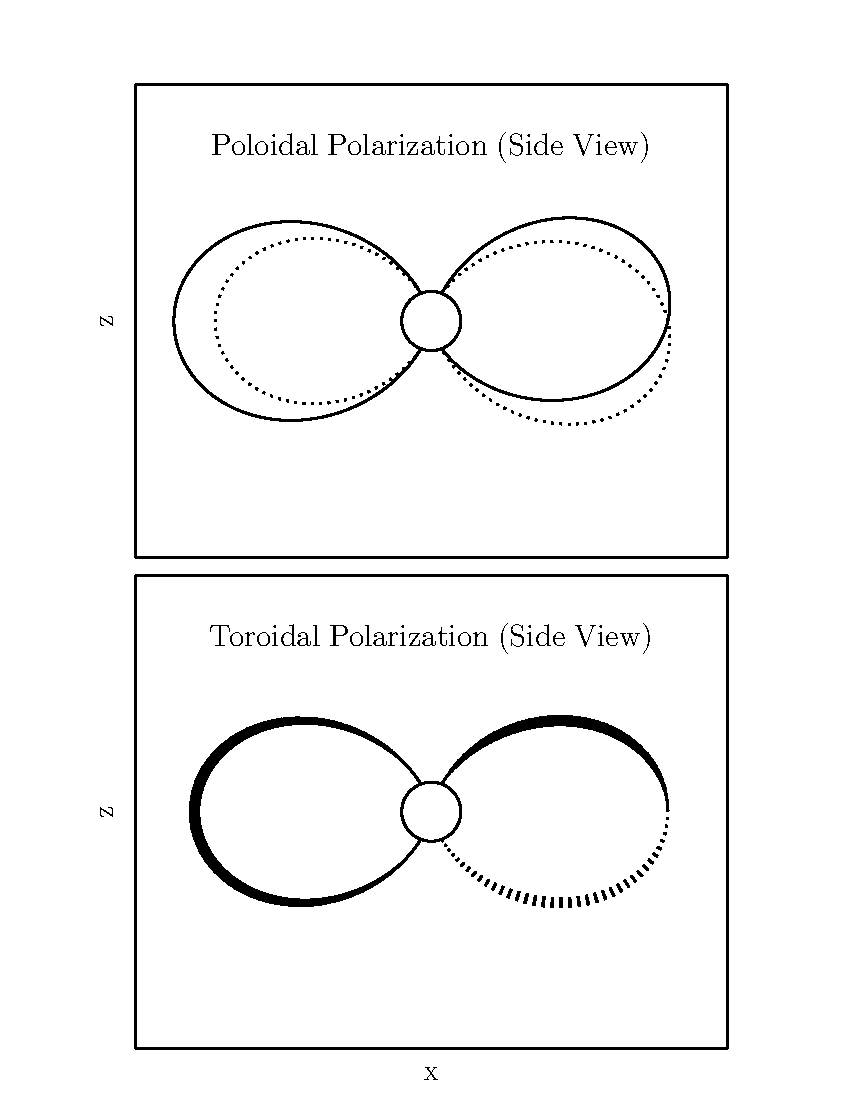
\includegraphics[width=\textwidth]{figures/polarizations.pdf}
\end{columns}

\end{frame}

% -----------------------------------------------------------------------------
% -----------------------------------------------------------------------------
% -----------------------------------------------------------------------------

\begin{frame}
\frametitle{Azimuthal Modenumber}

\begin{wideitemize}
\item Small azimuthal modenumber means the wave extends broadly around the equator. 
\item Large modenumber means the wave could fit many times around the equator. 
\item Small-\azm and large-\azm waves behave differently. 
\end{wideitemize}

\vfill

\centerline{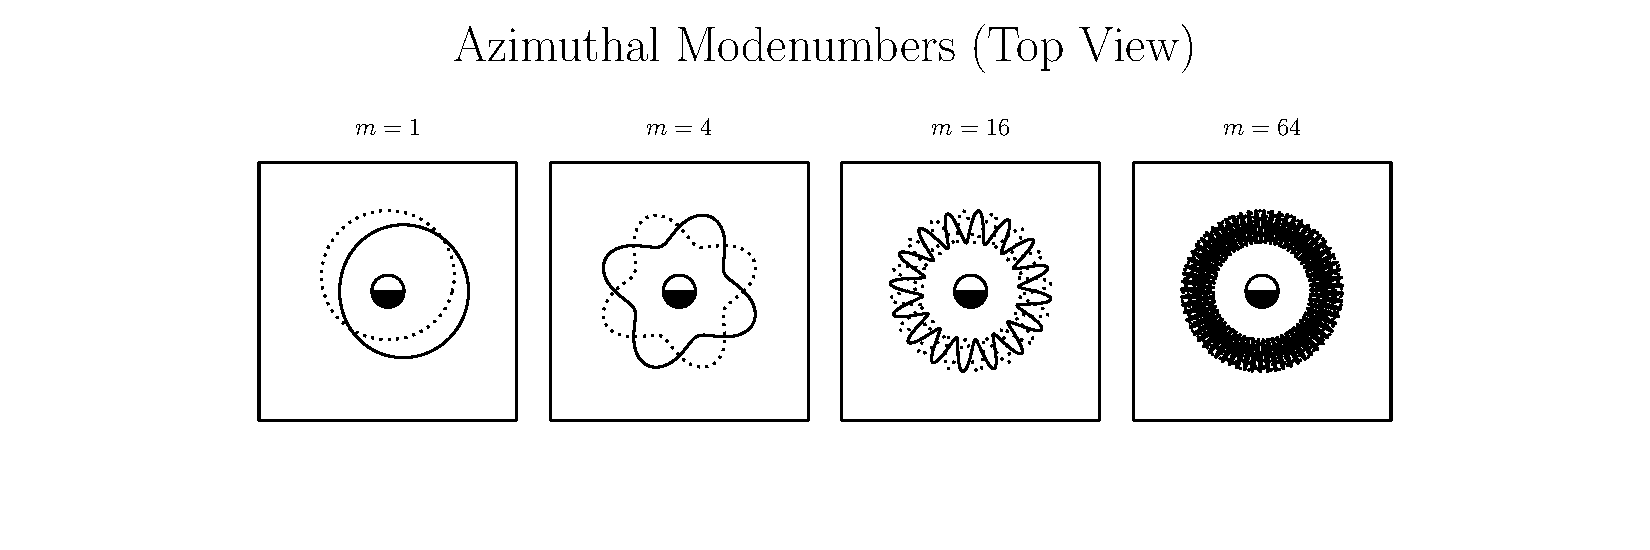
\includegraphics[width=1.2\textwidth]{figures/modenumber.pdf}}

%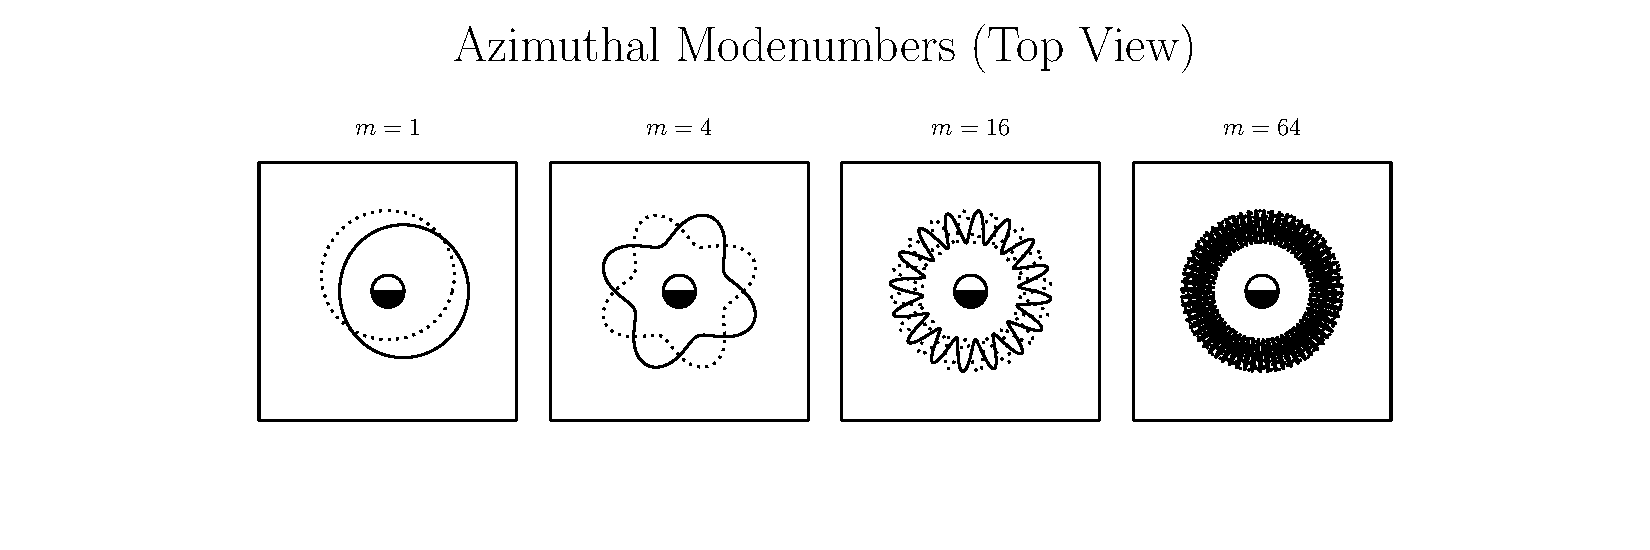
\includegraphics[width=\textwidth]{figures/modenumber.pdf}

\end{frame}

% -----------------------------------------------------------------------------
% -----------------------------------------------------------------------------
% -----------------------------------------------------------------------------

\begin{frame}
\frametitle{Pc4s and Giant Pulsations}

\begin{wideitemize}
\item Pc4 pulsations (\SIrange{7}{22}{\mHz}) resonate at auroral latitudes. 
\item They interact with trapped energetic particles. 
\item Giant pulsations are a small, distinctive subset of Pc4s.  
\end{wideitemize}

\vfill

\begin{center}
IAGA Frequency Bands [Jacobs, 1964]
\begin{tabular}{ @{\extracolsep{\fill}} cccccc @{\extracolsep{\fill}} }
  \hline
  & Pc1 & Pc2 & Pc3 & Pc4 & Pc5 \\
  \hline
  Period (\si{\second}) & 0.2--5    & 5--10    & 10--45  & 45--150 & 150--600 \\
  Frequency (\si{\mHz}) & 200--5000 & 100--200 & 22--100 & 7--22   & 2--7     \\
  \hline
\end{tabular}
\end{center}

\end{frame}

% =============================================================================
% ======================================================================= Model
% =============================================================================

\section{Numerical Model}

% -----------------------------------------------------------------------------
% -----------------------------------------------------------------------------
% -----------------------------------------------------------------------------

\begin{frame}
\frametitle{``Tuna Half'' Dimensional Model}

\begin{columns}
\column{0.33\textwidth}
\begin{wideitemize}
\item Near Earth, at high \azm, 3D is too expensive. 
\item Simplifying assumption: 2D grid, fields go as $\exp\arg{i \azm \phi}$. 
\item Then $\dd{\phi} \rightarrow i\azm$ allows 3D fields and 3D derivatives. 
\end{wideitemize}
\column{0.67\textwidth}
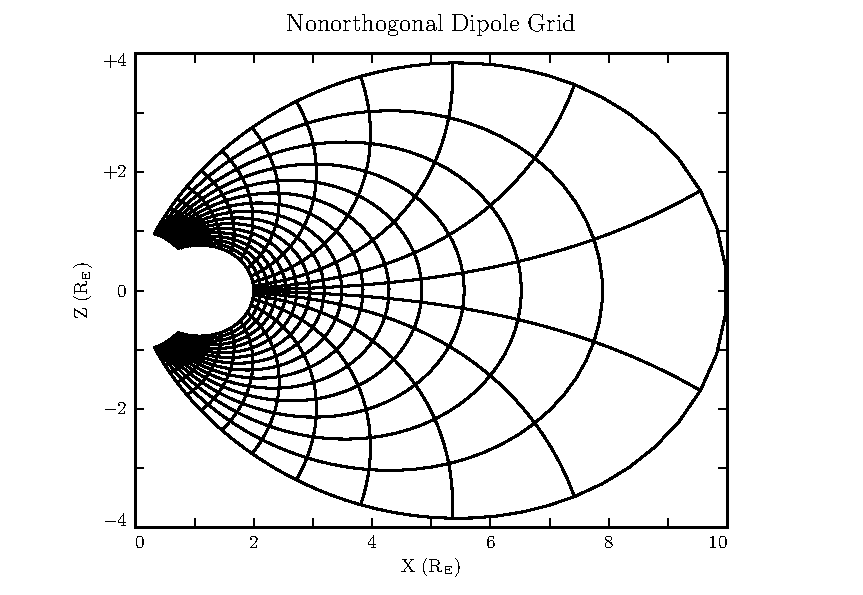
\includegraphics[width=\textwidth]{figures/grid.pdf}
\end{columns}

\end{frame}

% -----------------------------------------------------------------------------
% -----------------------------------------------------------------------------
% -----------------------------------------------------------------------------

\begin{frame}
\frametitle{Physical Parameter Profiles}

\begin{wideitemize}
\item Height-resolved conductivity from Kelley, modified by Lysak. 
\item Plasma density, including the plasmasphere. 
\item \Alfven speed from dipole field and density: $\va \equiv \frac{B}{\sqrt{\mz \rho}}$
\item Four profiles: active day, quiet day, active night, quiet night. 
\end{wideitemize}

\vfill

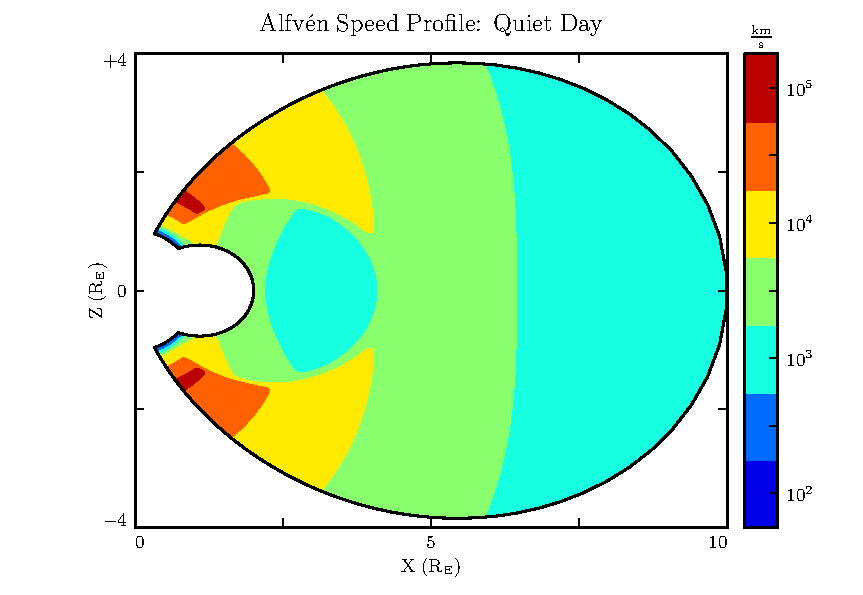
\includegraphics[width=0.5\textwidth]{figures/va_2.pdf}%
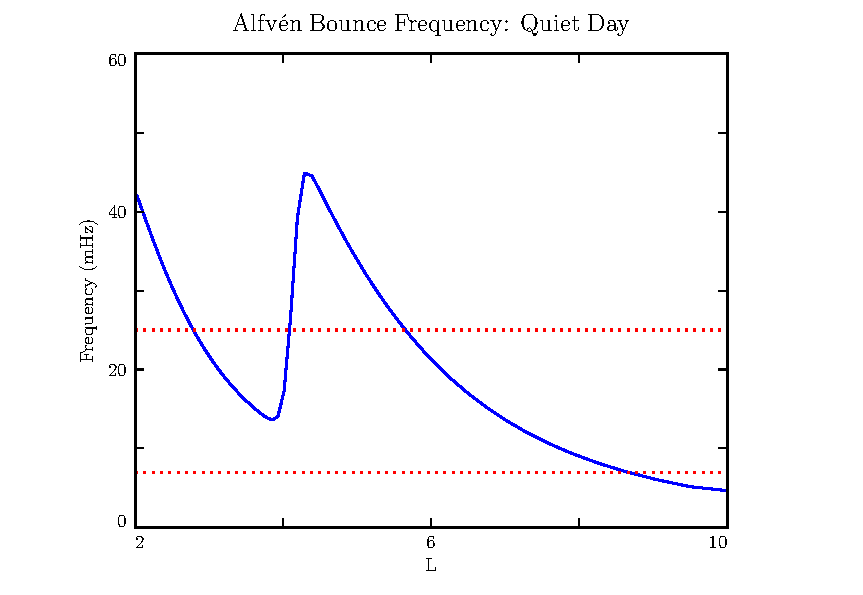
\includegraphics[width=0.5\textwidth]{figures/fa_2.pdf}%

\end{frame}

% -----------------------------------------------------------------------------
% -----------------------------------------------------------------------------
% -----------------------------------------------------------------------------

\begin{frame}
\frametitle{Driving --- Compression or Current?}

\begin{wideitemize}
\item At high \azm, driving at the outer boundary doesn't work. 
\item Tuna drives by perturbing the ring current instead. 
\end{wideitemize}

\vfill

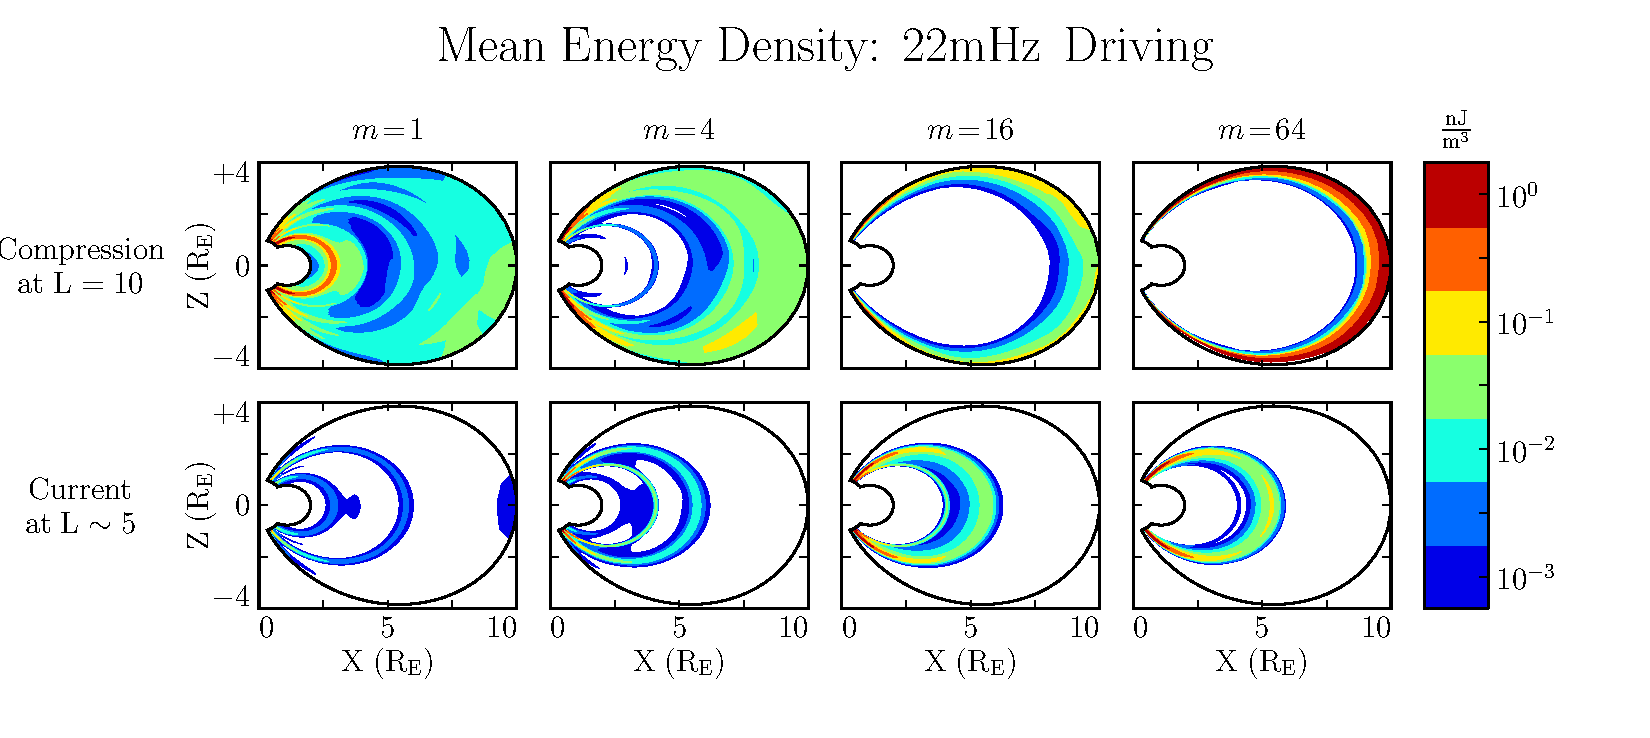
\includegraphics[width=\textwidth]{figures/drivers.pdf}%

\end{frame}

% -----------------------------------------------------------------------------
% -----------------------------------------------------------------------------
% -----------------------------------------------------------------------------

\begin{frame}
\frametitle{Maxwell's Equations}

Electric fields are updated using \amplaw and \ohmlaw:
\begin{align*}
  \tensor{\epsilon} \cdot \tfrac{\partial}{\partial t} \vec{E} = \tfrac{1}{\mz} \curl{B} - \vec{J} - \tensor{\sigma} \cdot \vec{E}
\end{align*}

Let $ \quad \tensor{V}^2 \equiv \frac{1}{\mz} \tensor{\epsilon}^{-1} \quad $ and $ \quad \tensor{\Omega} \equiv \tensor{\epsilon}^{-1} \cdot \tensor{\sigma} \quad $ so
\begin{align*}
  \lr{ \tensor{\Omega} + \tensor{ \mathbb{I} } \tfrac{\partial}{\partial t} } \cdot \vec{E} &= \tensor{V}^2 \cdot \big( \curl{B} - \mz \vec{J} \big)
\end{align*}

Which can be solved with an integrating factor: 
\begin{gather*}
  \highlight{\vec{E} \assign \exp \arg{ -\tensor{\Omega} \, \dt } \cdot \vec{E} +
    \dt \, \exp \arg{ -\tensor{\Omega} \, \tfrac{\dt}{2} } \cdot
    \tensor{V}^2 \cdot \big( \curl{B} - \mz \vec{J} \big)}
\end{gather*}

Magnetic fields are updated using \farlaw:
\begin{align*}
  \tfrac{\partial}{\partial t} \vec{B} &= -\curl{E} &
  & \text{so} &
  &\highlight{ \vec{B} \assign \vec{B} - \dt \, \curl{E} }
\end{align*}

\end{frame}

% -----------------------------------------------------------------------------
% -----------------------------------------------------------------------------
% -----------------------------------------------------------------------------

\begin{frame}
\frametitle{Coupling to the Atmosphere}

\begin{wideitemize}
\item Assume a perfectly-insulating atmosphere: $\curl{B} = 0$.  
\item From Maxwell's equations, $\div{B} = 0$. 
\item Then $\nabla^2\Psi = 0$ where $\nabla \Psi = \vec{B}$. 
\item Solution at the top of the atmosphere is a boundary condition:
\begin{align*}
  \tensor{\Sigma} \cdot \vec{E} &= \frac{1}{\mz} \,
    \displaystyle\lim_{\dr \rightarrow 0} \, \bigg[ \, \hat{r} \times \vec{B}
    \, \bigg|^{R_I + \dr}_{R_I - \dr}
\end{align*}
\item Solution at the bottom of the atmosphere gives ground signatures. 
\end{wideitemize}

\end{frame}

% =============================================================================
% ===================================================================== Results
% =============================================================================

\section{Numerical Results}

% -----------------------------------------------------------------------------
% -----------------------------------------------------------------------------
% -----------------------------------------------------------------------------

\begin{frame}
\frametitle{Snapshots of a Low-\azm Simulation}

\begin{wideitemize}
\item Poloidal and compressional waves are blobby. 
\item Toroidal waves are sharply defined. 
\item All components are similar in magnitude. 
\end{wideitemize}

\vfill

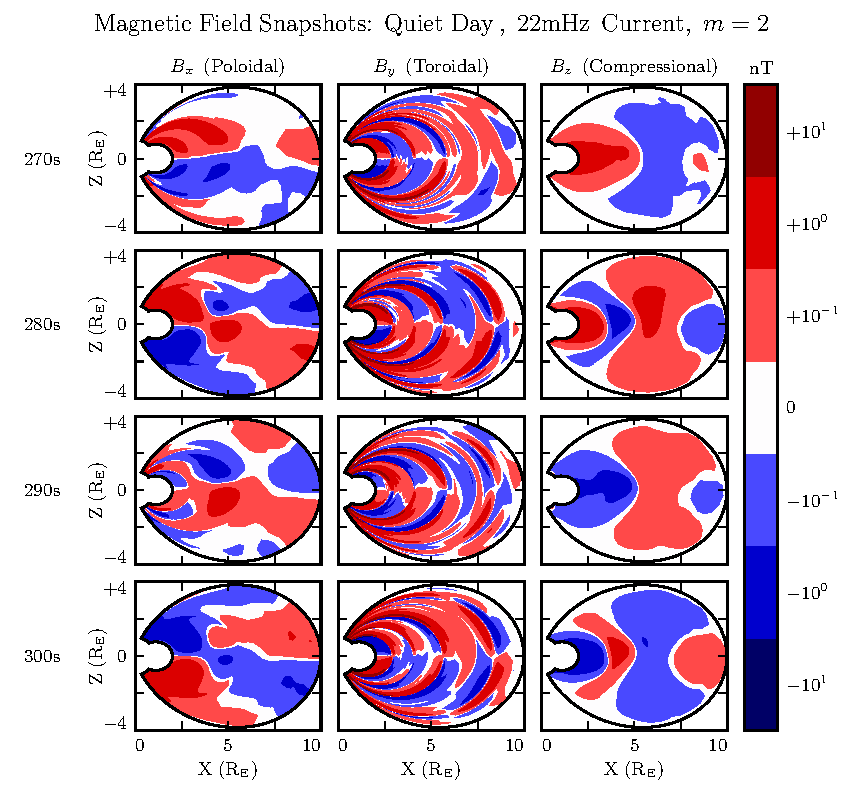
\includegraphics[width=\textwidth]{figures/snapshot_smallm.pdf}

\end{frame}

% -----------------------------------------------------------------------------
% -----------------------------------------------------------------------------
% -----------------------------------------------------------------------------

\begin{frame}
\frametitle{Snapshots of a High-\azm Simulation}

\begin{wideitemize}
\item Waves are barely compressional. 
\item Little energy crosses field lines. 
\item Poloidal waves are less smeared than at $\azm=2$, but still not as sharp as toroidal waves. 
\end{wideitemize}

\vfill

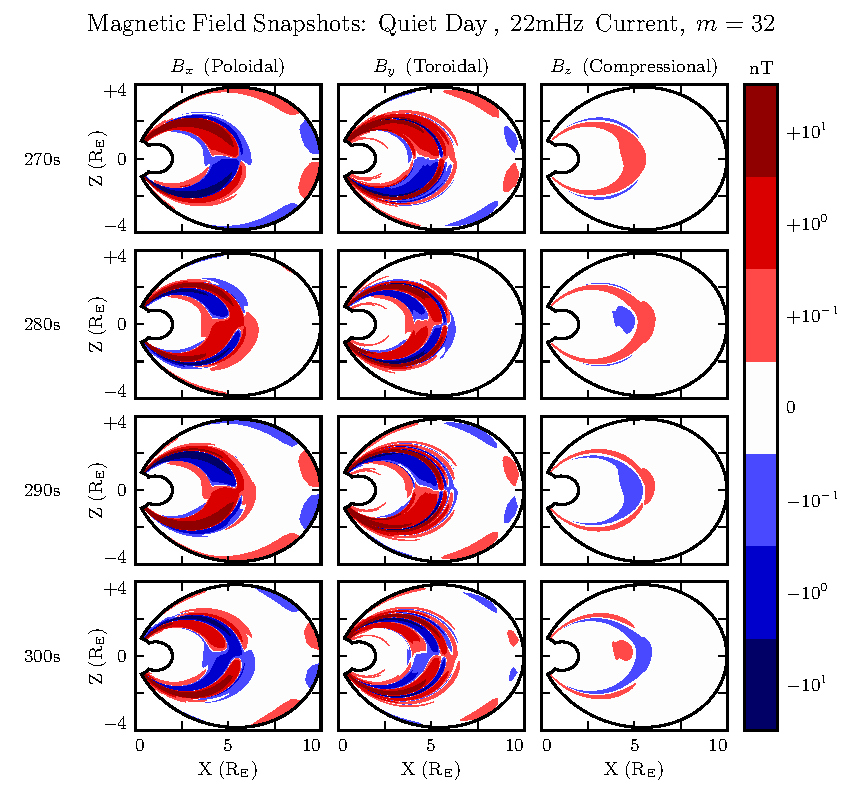
\includegraphics[width=\textwidth]{figures/snapshot_bigm.pdf}

\end{frame}

% -----------------------------------------------------------------------------
% -----------------------------------------------------------------------------
% -----------------------------------------------------------------------------

\begin{frame}
\frametitle{Poloidal-to-Toroidal Rotation}

\begin{wideitemize}
\item Polarization rotates over time from poloidal to toroidal. 
\item The rotation is slower at large \azm. 
\end{wideitemize}

\vfill

\begin{columns}
\column{0.5\textwidth}
\vfill
\begin{overpic}[width=\textwidth]{figures/mann_1995.png}
 \put (0, 1) {\tiny\textcolor{black}{\;Mann and Wright, 1995}}
\end{overpic}%
\column{0.5\textwidth}
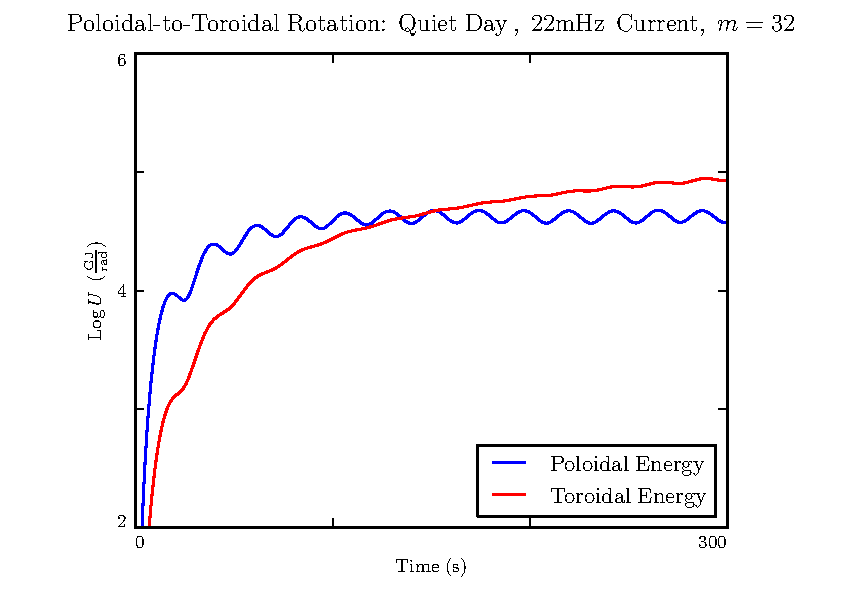
\includegraphics[width=\textwidth]{figures/rotate.pdf}
\vfill
\end{columns}

\end{frame}

% -----------------------------------------------------------------------------
% -----------------------------------------------------------------------------
% -----------------------------------------------------------------------------

\begin{frame}
\frametitle{Resonance and Rotation on the Dayside}

\begin{wideitemize}
\item Poloidal-to-toroidal rotation is fast compared to dissipation. 
\item Toroidal energy accumulates only where resonant. 
\item At small \azm, energy escapes to the outer boundary. 
\end{wideitemize}

\vfill 

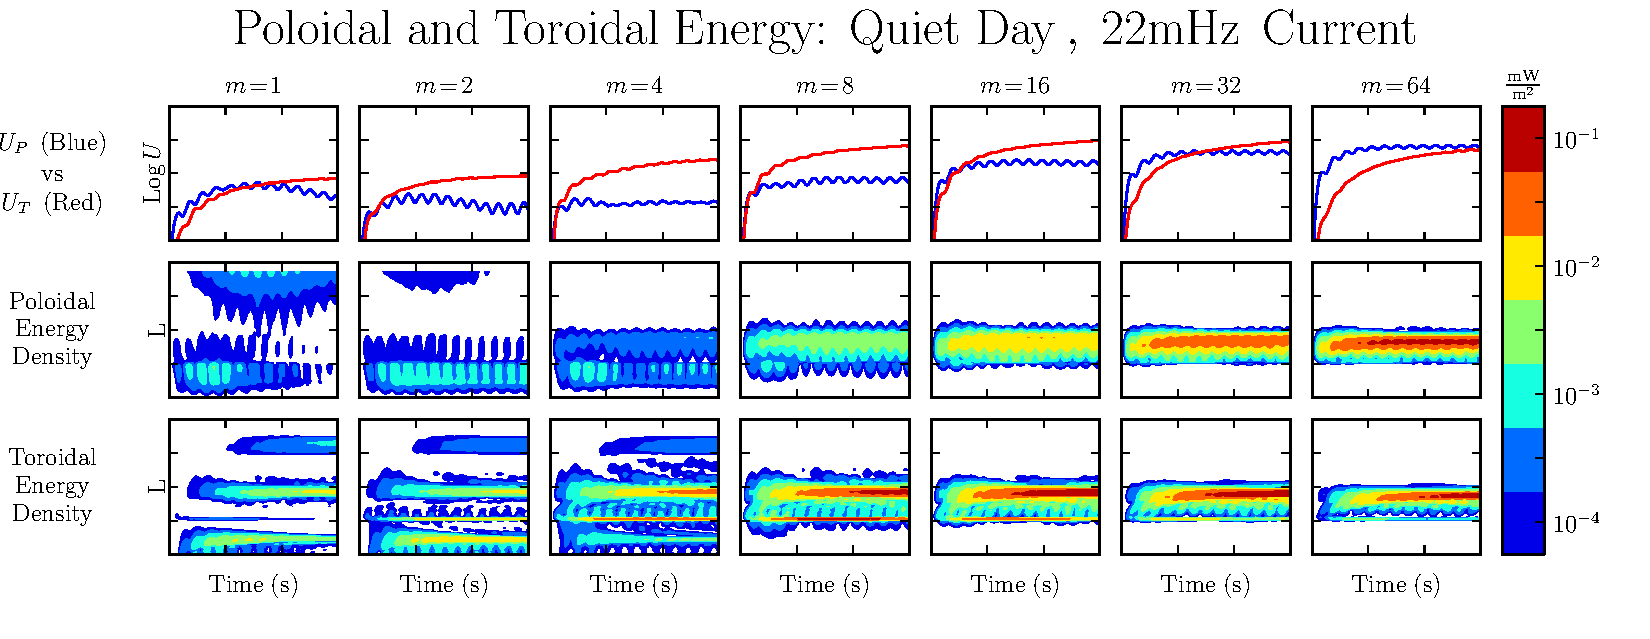
\includegraphics[width=\textwidth]{figures/energy_day.pdf}

\end{frame}

% -----------------------------------------------------------------------------
% -----------------------------------------------------------------------------
% -----------------------------------------------------------------------------

\begin{frame}
\frametitle{Resonance and Rotation on the Nightside}

\begin{wideitemize}
\item The nightside ionosphere is much less conductive than the dayside ionosphere. 
\item No accumulation of energy over multiple drive periods. 
\item At high \azm, dissipation is faster than poloidal-to-toroidal rotation. 
\end{wideitemize}

\vfill

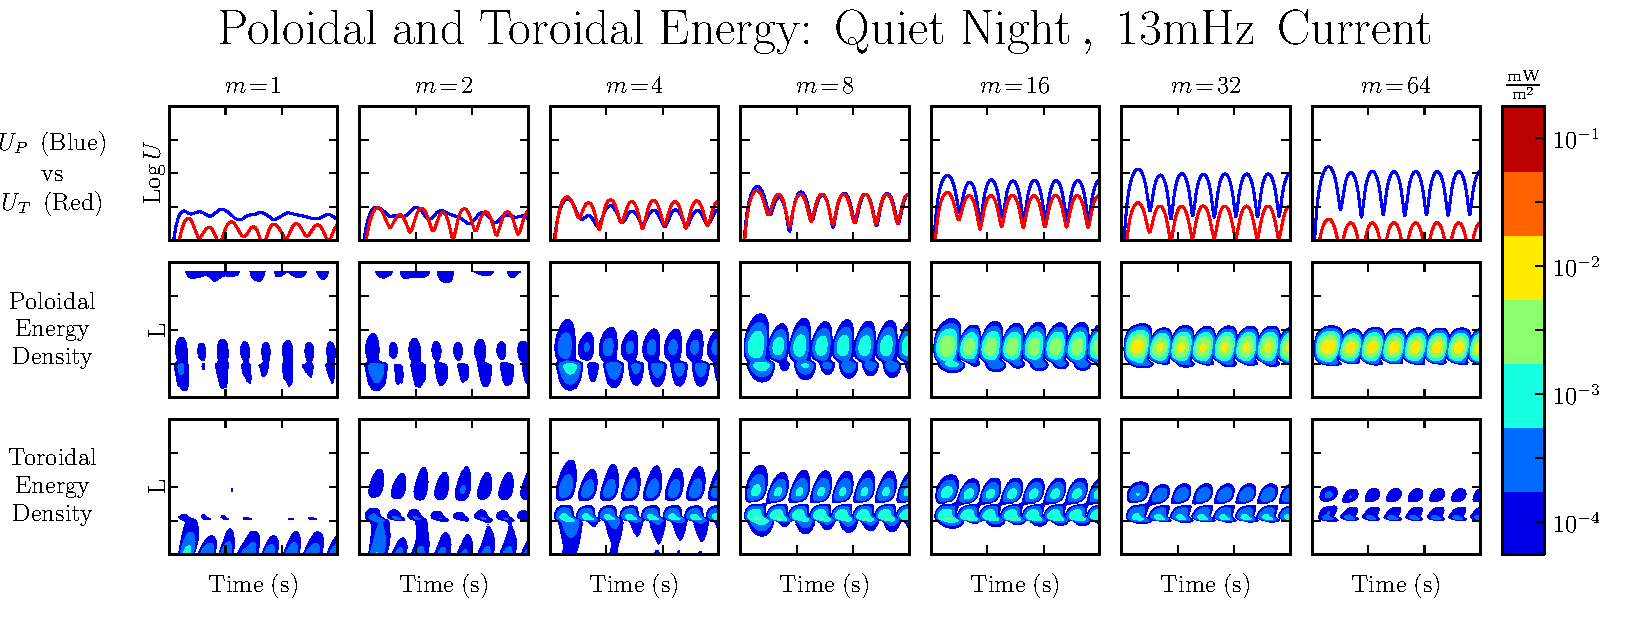
\includegraphics[width=\textwidth]{figures/energy_night.pdf}

\end{frame}

% -----------------------------------------------------------------------------
% -----------------------------------------------------------------------------
% -----------------------------------------------------------------------------

\begin{frame}
\frametitle{Ground Signatures and Giant Pulsations}

\begin{wideitemize}
%\item Ground signatures are the most convenient way to compare numerical results to observations. 
\item Peak at $\azm = 16$ to $32$, near \SI{65}{\degree} latitude. 
\item Counterclockwise at low latitude, clockwise at high latitude. 
\item It seems these properties are not unique to giant pulsations! 
\end{wideitemize}

\vfill

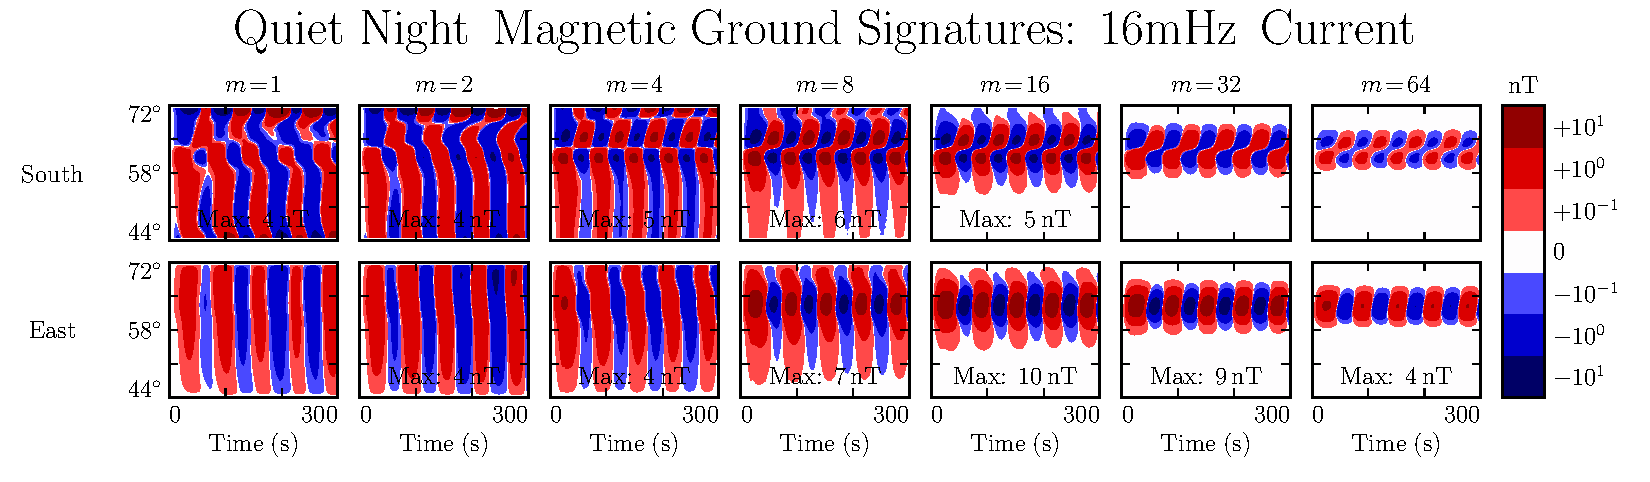
\includegraphics[width=\textwidth]{figures/ground_4.pdf}%

\end{frame}

% -----------------------------------------------------------------------------
% -----------------------------------------------------------------------------
% -----------------------------------------------------------------------------

\begin{frame}
\frametitle{Results from the Numerical Model}

\begin{wideitemize}
\item Toroidal frequencies depend sharply on $L$ because toroidal FLRs are sharp in $L$ --- unlike poloidal FLRs, which are smeared. 
\item At least in terms of \azm, latitude, and chirality, giant pulsations are not as distinctive as they are made out to be. 
\item Poloidal-to-toroidal rotation is fast --- the poloidal mode is a significant source for same-harmonic toroidal waves. 
\item Resonance on the nightside is significantly impeded by Joule dissipation in the ionosphere.  
\end{wideitemize}

\end{frame}

% =============================================================================
% ======================================================================== RBSP
% =============================================================================

\section{Van Allen Probe Observations}

% -----------------------------------------------------------------------------
% -----------------------------------------------------------------------------
% -----------------------------------------------------------------------------

\begin{frame}
\frametitle{Comparison to Observational Data?}

\begin{wideitemize}
\item How does the spatial distribution of giant pulsations compare to that of odd poloidal Pc4s overall?
\item How does the distribution of odd toroidal Pc4s compare to that of odd poloidal Pc4s?
\item How about even toroidal and even poloidal Pc4s?
\item We can address these questions with the Van Allen Probes. 
\end{wideitemize}

\end{frame}

% -----------------------------------------------------------------------------
% -----------------------------------------------------------------------------
% -----------------------------------------------------------------------------

\begin{frame}
\frametitle{Distribution of Usable Data}


\begin{columns}
\column{0.33\textwidth}
\begin{wideitemize}
\item Data spans October 2012 to August 2015. 
\item Nightside has been sampled twice at apogee. 
\item Full 3D fields computed per $\vec{E} \cdot \vec{B} = 0$, about half the data gets tossed.
\end{wideitemize}
\column{0.67\textwidth}
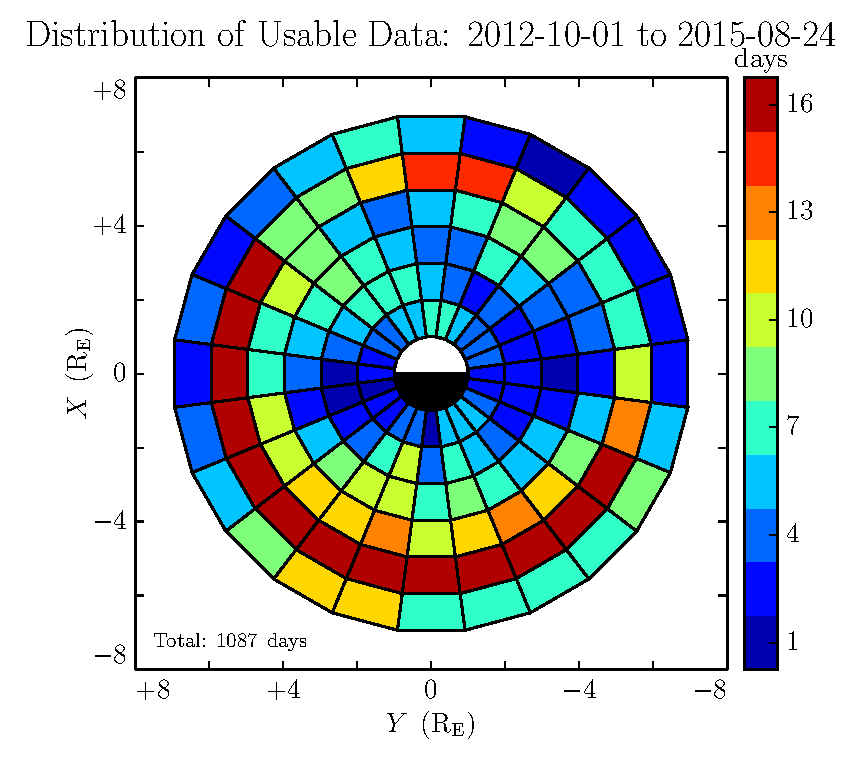
\includegraphics[width=\textwidth]{figures/pos_all_sharp.pdf}
\end{columns}

\end{frame}

% -----------------------------------------------------------------------------
% -----------------------------------------------------------------------------
% -----------------------------------------------------------------------------

\begin{frame}
\frametitle{Event Selection}

\begin{columns}
\column{0.33\textwidth}
\begin{wideitemize}
\item Split data into half-hour events. 
\item Compute Poynting flux spectrum. 
\item Threshold on frequency, magnitude, etc. 
\item Classify events by polarization and harmonic. 
\end{wideitemize}
\column{0.67\textwidth}
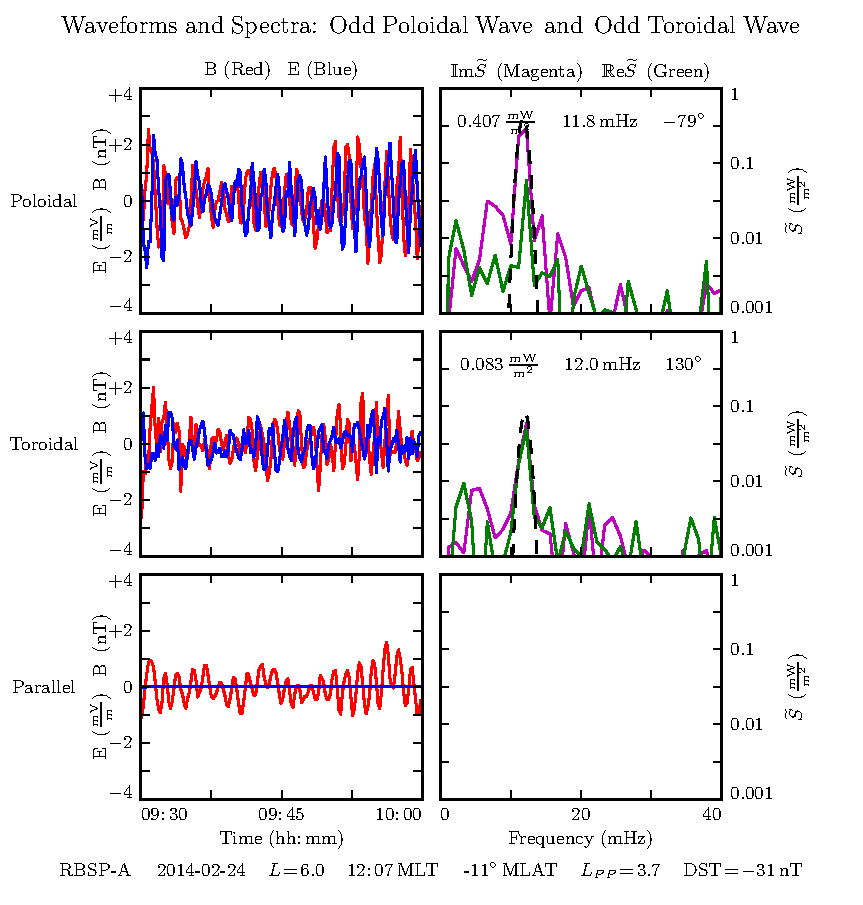
\includegraphics[width=\textwidth]{figures/sample_event_phase.pdf}
\end{columns}

\end{frame}

% -----------------------------------------------------------------------------
% -----------------------------------------------------------------------------
% -----------------------------------------------------------------------------

\begin{frame}
\frametitle{Pc4 Observation Rate}

\begin{columns}
\column{0.33\textwidth}
\begin{wideitemize}
\item Peak observation rate at noon.  
\item Fewest events at dusk. 
\item Stragglers near midnight. 
\item Generally consistent with previous surveys of Pc4 events. 
\end{wideitemize}
\column{0.67\textwidth}
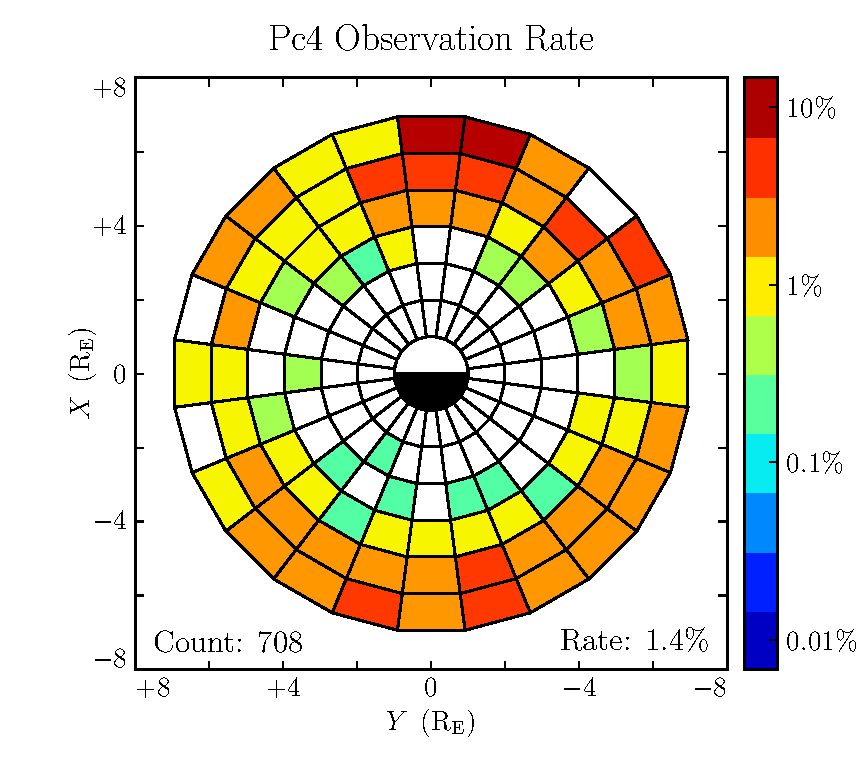
\includegraphics[width=\textwidth]{figures/rate_all_sharp.pdf}
\end{columns}

\end{frame}

% -----------------------------------------------------------------------------
% -----------------------------------------------------------------------------
% -----------------------------------------------------------------------------

\begin{frame}
\frametitle{Pc4 Observation Rate by Mode}

\begin{columns}
\column{0.33\textwidth}
Questions from before:

\vspace{5pt}

\begin{wideitemize}
\item Where are odd poloidal Pc4s compared to giant pulsations?
\item Where are odd toroidal Pc4s compared to odd poloidal Pc4s?
\item How about even toroidal and even poloidal Pc4s?
\end{wideitemize}
\column{0.67\textwidth}
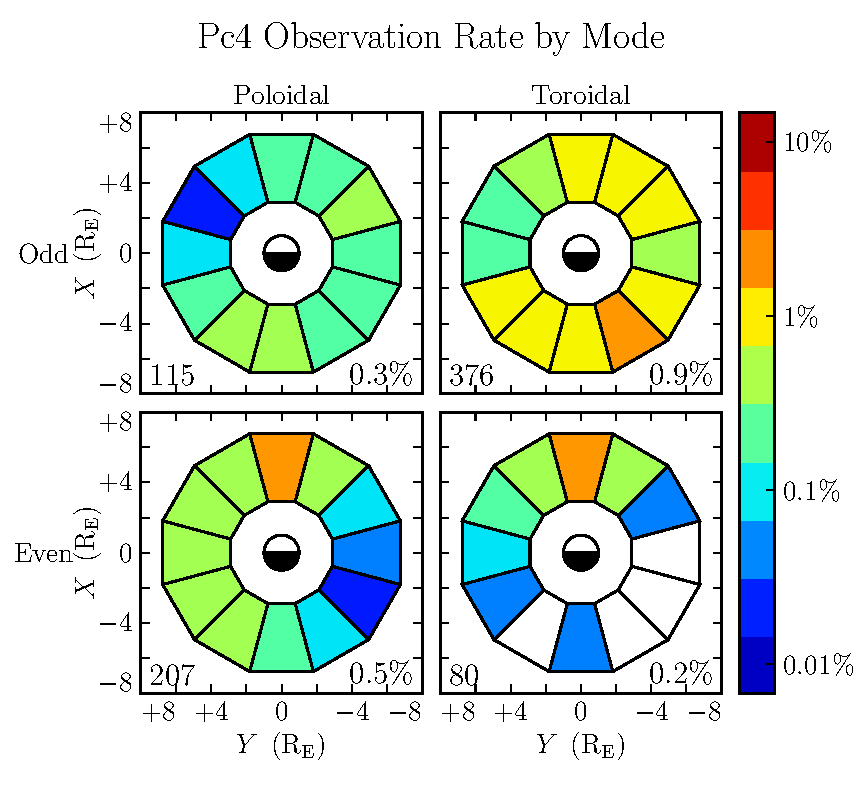
\includegraphics[width=\textwidth]{figures/mode_all.pdf}
\end{columns}

\end{frame}

% -----------------------------------------------------------------------------
% -----------------------------------------------------------------------------
% -----------------------------------------------------------------------------

\begin{frame}
\frametitle{Phase Distribution of Pc4 Events}

\vfill

\begin{columns}
\column{0.33\textwidth}
\begin{wideitemize}
\item Perfect standing waves have a phase of $\pm\SI{90}{\degree}$. 
\item The further from $\pm\SI{90}{\degree}$, the shorter the wave lifetime. 
\item Direct phase measurements are new and exciting! 
\end{wideitemize}
\column{0.67\textwidth}
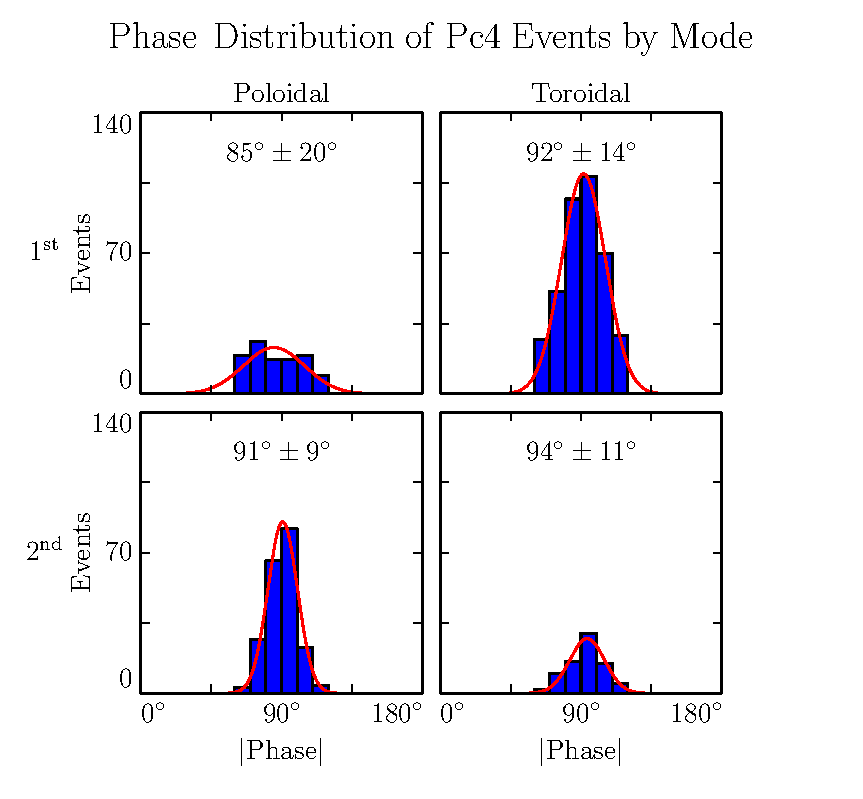
\includegraphics[width=\textwidth]{figures/phase.pdf}
\end{columns}

%\begin{wideitemize}
%\item Estimate wave lifetime from characteristic values $B$, $E$, and $R$:
%\begin{align*}
%  \tau &= \frac{BR}{2 E \cos\varphi} &
%  & \text{where} &
%  \varphi \equiv \arctan\frac{ \imag\dft{S} }{ \real\dft{S} }
%\end{align*}
%\item Standing waves: $\varphi = \pm\SI{90}{\degree}$. Traveling waves: $\varphi = \SI{0}{\degree}$ or \SI{180}{\degree}. 
%\item Odd modes are spread more from $\pm\SI{90}{\degree}$, at least at the equator. 
%\end{wideitemize}
%\vfill
%\centerline{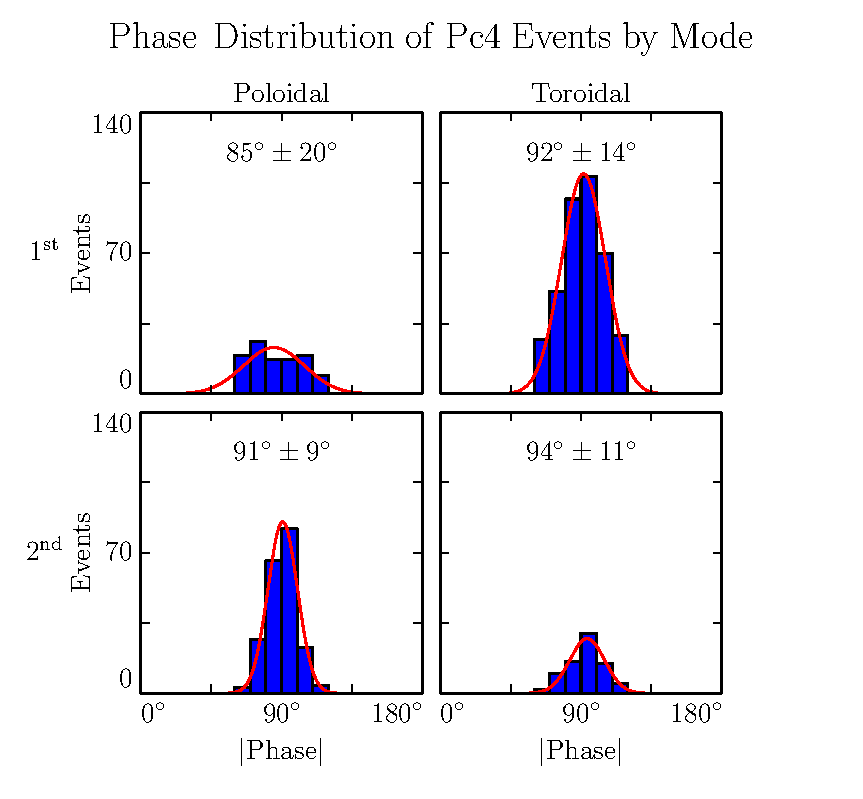
\includegraphics[width=1.2\textwidth]{figures/phase.pdf}}

\end{frame}

% =============================================================================
% ================================================================== Conclusion
% =============================================================================

\section{Conclusion}

% -----------------------------------------------------------------------------
% -----------------------------------------------------------------------------
% -----------------------------------------------------------------------------

\begin{frame}
\frametitle{Summary}

\begin{wideitemize}
\item Pc4s and giant pulsations have been shown to exhibit a mishmash of heretofore-unrelated properties. 
\item Tuna is a new two-and-a-half-dimensional simulation created with these waves in mind. 
\item Numerical results from Tuna suggest novel connections between several FLR properties. 
\item A survey of Van Allen Probes data shows good agreement with numerical results. 
\end{wideitemize}

\end{frame}

% -----------------------------------------------------------------------------
% -----------------------------------------------------------------------------
% -----------------------------------------------------------------------------

\begin{frame}
\frametitle{Thanks!}

\begin{columns}
\column{0.33\textwidth}
Committee:
\column{0.34\textwidth}
Funding:
\column{0.33\textwidth}
Collaborators:
\end{columns}

\begin{columns}
\column{0.33\textwidth}
\begin{wideitemize}
\item Bob Lysak (Advisor)
\item Cindy Cattell (Chair)
\item Tom Jones
\item Lindsay Glesener
\end{wideitemize}
\column{0.34\textwidth}
\begin{wideitemize}
\item NSF grant AGS-1405383
\item UMN OVPR
\item NASA grant NNX12AD14G
\item GEM Student Support
\end{wideitemize}
\column{0.33\textwidth}
\begin{wideitemize}
\item John Wygant
\item Dai Lei
\item Ian Mann
\item Aaron Breneman
\item Scott Thaller
\item Sheng Tian
\end{wideitemize}
\end{columns}

\end{frame}

% =============================================================================
% =============================================================== Backup Slides
% =============================================================================

\backupbegin
\section{Backup Slides}

% -----------------------------------------------------------------------------
% -----------------------------------------------------------------------------
% -----------------------------------------------------------------------------

\begin{frame}
\frametitle{Estimating Current from Sym-H}

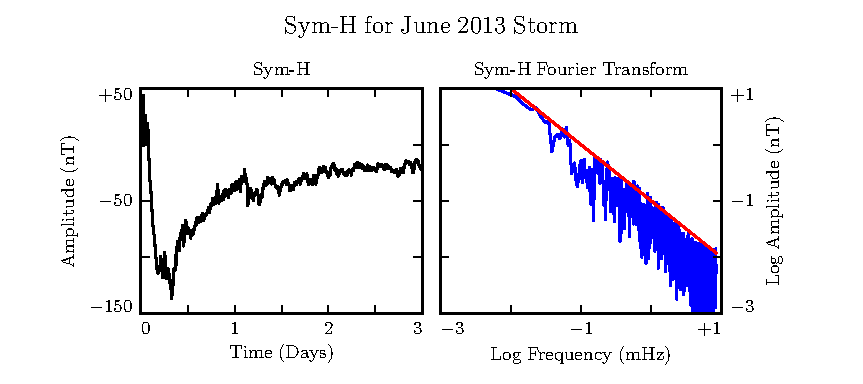
\includegraphics[width=\textwidth]{figures/symh.pdf}

\end{frame}

% -----------------------------------------------------------------------------
% -----------------------------------------------------------------------------
% -----------------------------------------------------------------------------

\begin{frame}
\frametitle{Van Allen Probe Sampling by Dst}

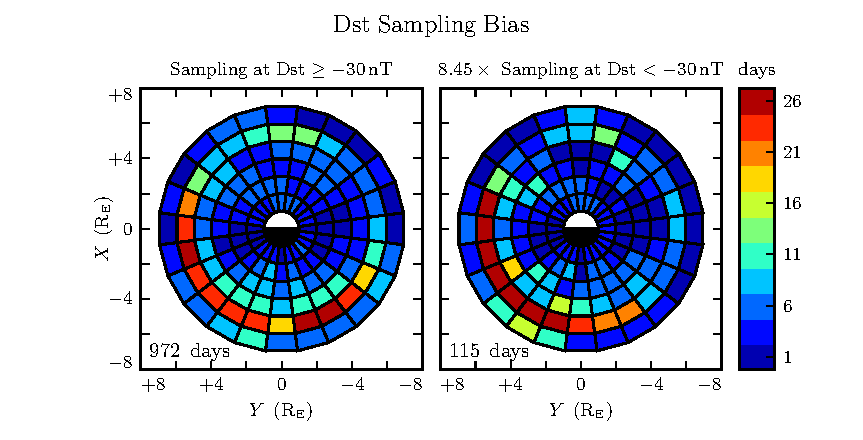
\includegraphics[width=\textwidth]{figures/dst_pos.pdf}

\end{frame}

% -----------------------------------------------------------------------------
% -----------------------------------------------------------------------------
% -----------------------------------------------------------------------------

\begin{frame}
\frametitle{Dawn-Dusk Asymmetry}

\begin{center}
\begin{overpic}[width=0.75\textwidth]{figures/grebowsky_1970.png}
 \put (0, 1) {\tiny\textcolor{black}{\;Grebowsky, 1970}}
\end{overpic}%
\end{center}

\end{frame}

% =============================================================================
% ================================================================ End Document
% =============================================================================

\backupend

\end{document}



